\documentclass[10pt, a4paper]{article}
% \usepackage[english]{babel}
\usepackage[brazilian]{babel}
\usepackage[utf8]{inputenc}
% \usepackage[T1]{fontenc}
\usepackage{lipsum}

% code
\usepackage{pythonhighlight}
\renewcommand{\lstlistingname}{Anexo} % Listing->Code
\usepackage{adjustbox}

% For subfigure use
\usepackage[font=small,labelfont=bf]{caption}
\usepackage{subcaption}

% Set page size and margins
% Replace `letterpaper' with`a4paper' for UK/EU standard size
\usepackage[a4paper,top=2cm,bottom=2cm,left=2cm,right=2cm,marginparwidth=2cm]{geometry}

% tabelas
\usepackage{array}
\usepackage{tabularx}
\usepackage{booktabs}

\usepackage{float}

% Useful packages
\usepackage{amsmath}
\usepackage{enumerate}

\usepackage{graphicx}
\usepackage[colorlinks=true, allcolors=blue]{hyperref}
\usepackage{cleveref}
%\usepackage[notransparent]{svg}
\newcommand{\crefrangeconjunction}{--}


\begin{document}

\def\TITLE{Trabalho 01}
\def\DISCIPLINE{MEC 2403 - Otimização e Algoritmos para Engenharia Mecânica}
\def\PROFESSOR{Ivan Menezes}
\def\AUTHOR{Pedro Henrique Cardoso Paulo}
\def\CONTACT{pedrorjpaulo.phcp@gmail.com}
\def\DATE{maio de 2023}

\title{\textbf{\TITLE} \\ \DISCIPLINE}
\author{\AUTHOR}
\date{\DATE}

\begin{titlepage}
      \begin{center}
          \vspace*{1cm}

          \Huge
          \textbf{\TITLE}

          \vspace{0.5cm}
          \LARGE
          \DISCIPLINE

          \vspace{1.5cm}

          \textbf{\AUTHOR \\ {\tt \CONTACT}}

          \vfill
          Professor: \PROFESSOR

          \vspace{0.8cm}

          
\includegraphics[width=0.2\textwidth]{../general/puc.jpg}

          \Large
          Departamento de Engenharia Mecânica\\
          PUC-RJ Pontifícia Universidade Católica do Rio de Janeiro\\
          \DATE

      \end{center}
  \end{titlepage}

\maketitle

\section{Introdução}

\subsection{Objetivos}

Esse é o entregável da \TITLE \ da disciplina \DISCIPLINE. Esse trabalho tem como objetivos:

\begin{enumerate}
  \item Aplicar os principais métodos de otimização sem restrição (OSR) implementados na \href{https://github.com/prj-phcp/MEC2403_Activities/blob/master/Lista2/Lista2.pdf}{Lista 02}
  \item Comparar os valores obtidos e número de passos para funções quadráticas e não quadráticas com o previsto pela literatura para cada método
  \item Aplicar os otimizadores em problemas complexos e testar sua escalabilidade
\end{enumerate}

Para atingir esse objetivo, este trabalho consistirá na realização de dois exercícios. O primeiro consistirá na aplicação dos
métodos de otimização a duas funções distintas, sendo a primeira quadrática e a segunda não. O segundo exercício consistirá 
na solução de um problema de inspiração física, capaz de ser solucionado pelo método dos elementos finitos.

\subsection{Links úteis}\label{links}

Nesta seção são listados alguns links e referências úteis para se entender o trabalho desempenhado.

\begin{enumerate}
  \item \href{https://web.tecgraf.puc-rio.br/~ivan/MEC2403/ProgMatematica_VazPereiraMenezes-Ago2012.pdf}{Apostila de programação matemática da disciplina}
  \item \href{https://github.com/prj-phcp/MEC2403_Activities}{GitHub usado para essa disciplina}
  \item \href{https://github.com/prj-phcp/MEC2403_Activities/blob/master/Trabalho1/Trabalho1.ipynb}{Notebook com o código para as figuras desse relatório}
  \item \href{https://github.com/prj-phcp/MEC2403_Activities/blob/master/Trabalho1/Derivadas.ipynb}{Notebook com o código para derivação simbólica das funções mais complexas}
  \item \href{https://github.com/prj-phcp/MEC2403_Activities/blob/master/packages}{Pasta com os códigos a serem aproveitados em todas as listas}
\end{enumerate}

\section{Materiais e métodos}

Nesta seção serão descritos os principais métodos de otimização aplicados neste estudo, tal como detalhes de sua implementação
em código Python.

\subsection{Otimização sem restrição (OSR)}

Otimização sem restrição consiste na busca de um mínimo de uma função $f(\mathbf{x})$ a partir de um processo iterativo partindo
de um ponto inicial $\mathbf{x_0}$. Tal como o nome sugere, nesta classe de problemas não há restrição quanto ao domínio da
função $f$, sendo o mínimo final obtido uma função do ponto inicial e dos algoritmos aplicados para a solução do problema.

Via de regra, todo algoritmo de otimização sem restrição consiste em um \textit{loop} dos seguintes passos, repetidos até que
dada condição de parada seja atingida:

\begin{enumerate}
  \item A partir de dada posição $\mathbf{x_i}$, determinar uma direção de busca $\mathbf{d_i}$ na qual o mínimo será procurado
  \item Executar bsca linear para determinar o passo $\alpha_i$ que leva ao ponto de mínimo na direção $\mathbf{d_i}$
  \item Atualizar o valor de posição $\mathbf{x_{i+1}} = \mathbf{x_i} + \alpha_i\mathbf{d_i}$
\end{enumerate}

A condição de parada típica para esses problemas é a condição necessária de primeira ordem, i.e. $|\mathbf{\nabla}f| < tol$.
Esta será a condição aplicada em todos os exercícios deste trabalho e, embora de fácil implementação nos casos em que o 
gradiente é conhecido, apresenta como desvantagens não garantir o atingimento de um mínimo global (problema comum a todos os
algoritmos de minimização) e de não garantir o atingimento de um mínimo (qualquer ponto crítico como máximos e pontos de sela
atenderiam à condição).

\subsection{Métodos de determinação de direção}

Nesta seção serão descritos os principais métodos de determinação de direção implementados neste estudo. Ressalta-se que no 
escopo deste trabalho, todos eles serão usados em todos os itens.

\subsubsection{Univariante}

É o método mais simples de seleção de direção que consiste em selecionar alternadamente as direções da base canônica como
como a direção de busca linear. tem a seu favor a simplicidade e a independência do conhecimento das derivadas da função,
mas apresenta como contras sua tendência a baixa eficiência e o fato de não haver garantias de que a direção proposta tem
sentido alinhado com um mínimo, exigindo checagem para valores de $\alpha$ negativos.

\subsubsection{Powell}

Método de otimização que, como o univariante, independe do conhecimento prévio de derivadas da função a ser otimizada. Sua
maior característica é o uso de direções Q-conjugadas para uma tentativa de ganho de performance quando comparado ao
univariante. Uma descrição simples do processo o método é apresentada a seguir:

\begin{enumerate}
  \item Começa-se com um conjunto de direções candidatas composto pelas canônicas\label{item:powell_1}
  \item É realizado um \textit{loop} nas direções candidatas\label{item:powell_2}
  \item Uma nova direção $\mathbf{d}$ é determinada pela diferença entre o ponto ao fim e ao início do \textit{loop}
  \item Uma otimização é realizada na direção $\mathbf{d}$. Essa direção é Q-conjugada.
  \item Caso ainda hajam direções canônicas na lista de candidatas, a primeira direção da lista é descartada e $\mathbf{d}$ é adicionada à lista. Retorna-se ao passo \ref{item:powell_2}
  \item Caso contrário, retorna-se ao item \ref{item:powell_1}
\end{enumerate}

A grande vantagem do método de Powell é que a aplicação de direções Q-conjugadas garante a convergência para funções quadráticas
no primeiro passo após termos apenas candidatas Q-conjugadas. Assim, para funções quadráticas, espera-se que o método convirja em
$(n+1)^2$ passos, onde $n$ é a dimensão do domínio da função.

\subsubsection{Steepest Descent}

Método que consiste em definir $\mathbf{d_i} =  - \mathbf{\nabla}f(\mathbf{x_i})$. A motivação para essa formulação é seguir a direção
que localmente leva ao mais rápido decréscimo do valor da função, sendo esta função o oposto do gradiente.

\subsubsection{Fletcher-Reeves}

Consiste na minimização da função $f$ por sua aproximação pro uma função quadrática. Esse método trabalha com direções Q-conjugadas após o
primeiro passo por meio da atualização das direções por meio da expressão $\mathbf{d_{i+1}} = -\mathbf{g_{i+1}} + \beta_i\mathbf{d_{i}}$, com $\mathbf{g_{i+1}}$
sendo o gradiente da função $f$. 
Para o método de Fletcher-Reeves, o valor de $\beta_i$ é calculado pela equação \ref{eq:frbeta}.

\begin{equation}\label{eq:frbeta}
  \beta_i = \frac{\mathbf{g^T_{i+1}}\mathbf{g_{i+1}}}{\mathbf{g^T_{i}}\mathbf{g_{i}}}
\end{equation}

Por trabalhar com a direção conjugada a partir do primeiro passo, no caso de uma função quadrática, espera-se que o método convirja em $(n+1)$
passos, onde $n$ é a dimensão do domínio da função.

\subsubsection{Newton-Raphson}

Método de segunda ordem que trabalha com direções conjugadas desde o primeiro passo, mas em contrapartida demanda conhecimento da Hessiana ($\mathbf{H}$)
da função, i.e. suas derivadas segundas. A direção é dada pela expressão $\mathbf{d_i} = (\mathbf{H}(f)_{\mathbf{x}=\mathbf{x_i}})^{-1}\mathbf{\nabla}f(\mathbf{x_i})$.
Converge em $n$ passos ou menos para funções quadráticas.

\subsubsection{BFGS}

Método de primeira ordem que tenta emular o comportamento de Nwton-Raphson sem a construção explícita de Hessiana. Para tal, é criada uma matriz $\mathbf{S}$ que é atualizada com
base nos valores de gradiente e ponto ao longo da corrida. Tente a convergir em $(n+1)$ passos ou menos pra funções quadráticas.
\subsection{Métodos de Busca Linear}

Nesta seção serão descritos brevemente os métodos de busca linear para a determinação de mínimos em dada direção.
Para os exercícios deste trabalho, apenas o método da seção áurea, com intervalo inicial determinado pelo passo constante
serão aplicados.
\subsubsection{Passo constante}

Método mais simples de busca linear, consiste em ir incrementando o valor de $\alpha$ por um valor constante até
chegarmos a um ponto em que a função comece a crescer. Muito usado para fins de determinar um intervalo inicial para
a busca por métodos mais eficientes.

Importante ter em mente que este método supõe que a direção de busca tem um sentido que aponta para o mínimo, de modo
que uma checagem de se isso é verdade é essencial caso o método de geração da direção não consiga garantir isso.

\subsubsection{Bisseção}

Método para busca do mínimo em um intervalo $[\alpha_{min}, \alpha_{max}]$ que consiste na divisão do intervalo sempre na metade
e descarte de parte dele. É feito iterativamente até que se atinja um valor de $\alpha_{max}-\alpha_{min}$ pré-determinado.

\subsubsection{Seção Áurea}

Método para busca do mínimo em um intervalo $[\alpha_{min}, \alpha_{max}]$ que consiste na divisão do intervalo em três
seções, com os valores intermediários dependendo da razão áurea. Uma das seções mais extremas é sempre descartada. 
É feito iterativamente até que se atinja um valor de $\alpha_{max}-\alpha_{min}$ pré-determinado, tendo o potencial de
ser mais eficiente numericamente que a bisseção por conta de sua formulação.

\subsection{Implementação em Python}

A implementação dos métodos se deu por meio da criação, em linguagem Python, de três objetos principais responsáveis por uma
parte do processo de otimização. A estrutura de classes final é resumida na Figura \ref{fig:classes}. Em termos de organização,
o código ficou quebrado em 3 arquivos principais, a saber:

\begin{itemize}
  \item {\tt \href{https://github.com/prj-phcp/MEC2403_Activities/blob/master/packages/steps.py}{steps.py}}: Arquivo contendo a classe {\tt GenericStep} 
  e suas subclasses. Seu código encapsula os métodos de busca linear que são responsáveis pela determinação do $\alpha$ e também a execução de checagens
  do sentido da direção proposta.
  \item {\tt \href{https://github.com/prj-phcp/MEC2403_Activities/blob/master/packages/functions.py}{functions.py}}: Arquivo contendo a classe {\tt SpecialFunction}
  e suas subclasses. A função dessa classe é encapsular em um único objeto a função, sua hessiana e seu gradiente para conveniência dos métodos. Cabe comentar que
  neste módulo também há a subclasse {\tt NumericalSpecialFunction} que tem por objetivo calcular numericamente gradientes e hessianas de funções usando o pacote 
  {\tt numdifftools}. Essa classe será usada para os testes de generalização apenas onde a derivação analítica for impossível ou muito custosa. 
  \item {\tt \href{https://github.com/prj-phcp/MEC2403_Activities/blob/master/packages/optimizers.py}{optimizers.py}}: Arquivo que contem a classe {\tt GenericOptimizer}
  e suas subclasses. É nesse arquivo que são definidos os procedimentos para iteração dos métodos, cálculo das direções e critérios de parada (tanto o gradiente quanto um
  numero máximo de iterações). Importante ressaltar que os objetos neste módulo esperam receber {\tt SpecialFunction} e {\tt GenericStep} para performar sua tarefa.
\end{itemize}

\begin{figure}[htpb]
  \centering
  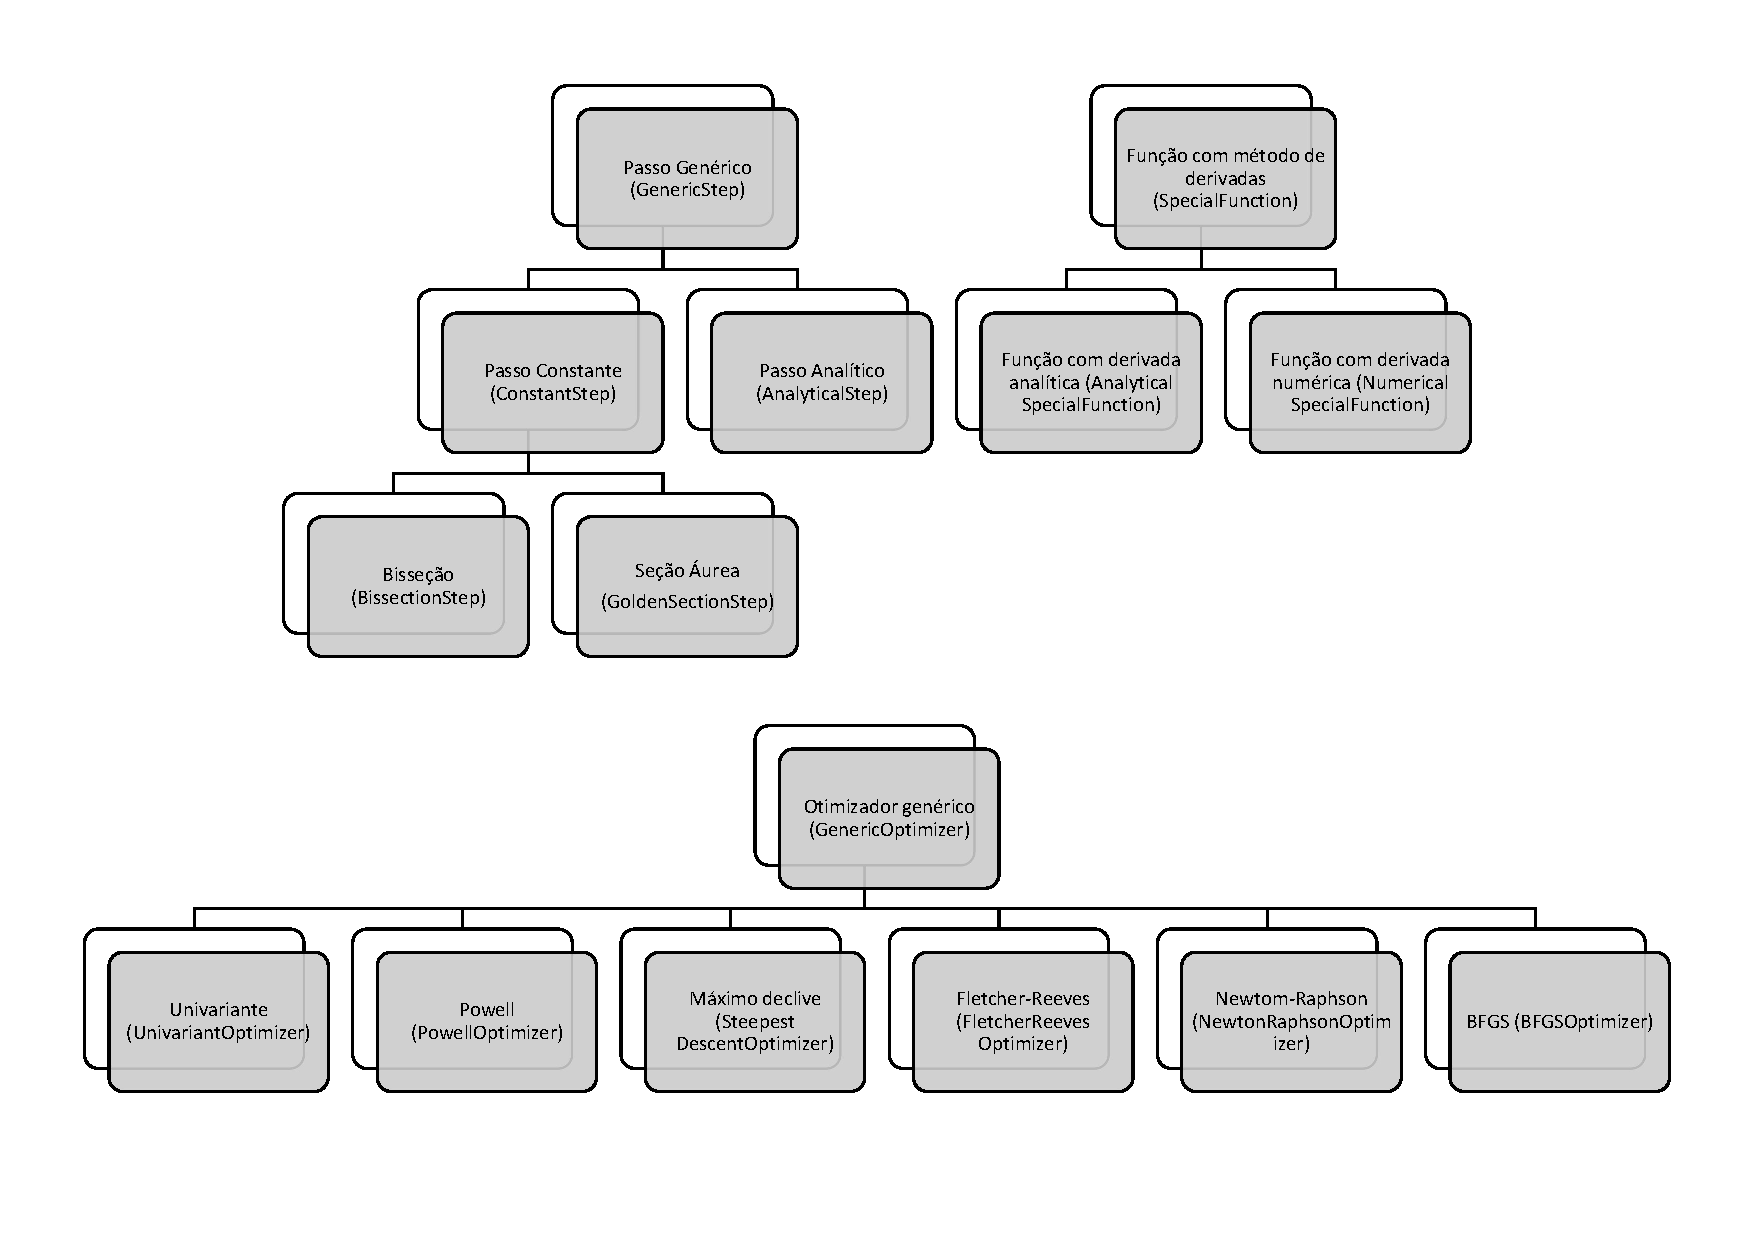
\includegraphics[width=0.8\textwidth]{../general/classes_full.pdf}
  \caption{Estrutura de classes implementada e heranças}
  \label{fig:classes}
\end{figure}

O uso desses classes para a execução das tarefas consiste em primeiramente, alocar os objetos de passo e otimizadores que gostaríamos de usar conforme exemplo abaixo:

\begin{python}
# Alocacao do Step
step = steps.GoldenSectionStep(da = 0.01, tol = 1e-8, check_direction=True, normalize=False)

#Alocacao dos optimizers
optimizrs = [
    ('Univariant', optimizers.UnivariantOptimizer(tol=1e-5)),
    ('Powell', optimizers.PowellOptimizer(tol=1e-5)),
    ('Steepest', optimizers.SteepestDescentOptimizer(tol=1e-5)),
    ('FletchRvs', optimizers.FletcherReevesOptimizer(tol=1e-5)),
    ('NewtnRaph', optimizers.NewtonRaphsonOptimizer(tol=1e-5)),
    ('BFGS', optimizers.BFGSOptimizer(tol=1e-5)),
]
\end{python}

Em seguida, a função de interesse é encapsulada em uma {\tt AnalyticalSpecialFunction}, junto com a definição
dos pontos iniciais e suas cores:

\begin{python}
# Definir f, grad, e hess
def f(x1, x2):

return x1**2 - 3*x1*x2 + 4*x2**2 + x1 - x2

def gradf(x1, x2):

return np.array(
    [ 2*x1 - 3*x2 + 1, 
    -3*x1 + 8*x2 - 1]
)

def hessf(x1, x2):

return np.array(
    [
    [ 2, -3],
    [-3,  8]
    ]
)

# Encapsular como SpecialFunction

f = functions.AnalyticalSpecialFunction(f, gradf, hessf)

# Definir pontos iniciais do processo

points = [
(np.array([2, 2]), 'r'),
(np.array([-1, -3]), 'b'),
]
\end{python}

Por fim, um \textit{loop} é executado por todos os métodos de otimização para determinar os 
mínimos e gerar os gráficos:

\begin{python}
item = 'a'

x = np.linspace(-6, 4, 100)
y = np.linspace(-6, 4, 100)
X, Y = np.meshgrid(x, y)
Z = f(X, Y)

levels =[0, 1, 2, 5, 7, 10, 20, 30, 40, 50]

for name, optimizer in optimizrs:
    fig, ax = plt.subplots(1,1, figsize=(5, 5))
    ax.contour(X, Y, Z, levels,cmap='rainbow')
    for p_inicial, color in points:
        t_init = datetime.datetime.now()
        p_final = optimizer(f, p_inicial, step)
        t_final = datetime.datetime.now()
        print(f'{name}: p_final = [{p_final[0]:.6f}, {p_final[1]:.6f}, {f(*p_final):.6f}].T. Execucao:{t_final - t_init}, {optimizer.iter} iteracoes')
        ax.plot(*p_inicial, f'{color}o')
        ax.text(p_inicial[0]-0.25, p_inicial[1]+0.25, f'$P_{{inic}} = [{p_inicial[0]}, {p_inicial[1]}]$', color=color)
        ax.plot(*p_final, 'ko')
        ax.text(p_final[0]-0.3, p_final[1]-0.5, f'$P_{{final}} = [{p_final[0]:.1f}, {p_final[1]:.1f}]$', color='k')
        cache = optimizer.get_history()
        for i in range(len(cache)-1):
            p_i = cache[i]
            p_f = cache[i+1]
            ax.quiver(p_i[0], p_i[1], p_f[0]-p_i[0], p_f[1]-p_i[1], color=color, angles='xy', scale_units='xy', scale=1)#, label='Passo completo')
    ax.grid()
    #ax.legend()
    ax.set_xlabel('$x_1$')
    ax.set_ylabel('$x_2$')
    ax.set_title(f'${name}$')
    fig.savefig(f'images/q1{item}_{name}.pdf')
\end{python}

\section{Questão 01}\label{sec:q01}

\subsection{Enunciado}

Implementar, usando o MATLAB ou Python, os métodos de otimização: (a) \textit{Univariante}; (b) \textit{Powell}; (c) \textit{Steepest Descent}; 
(d) \textit{Fletcher–Reeves}; (e) \textit{BFGS}; e (f) \textit{Newton–Raphson}. Adotar o método da Seção Áurea para a realização das buscas unidirecionais
(line search). Para verificação da convergência numérica, utilizar uma tolerância de $10^{-5}$. Em seguida, testar a sua implementação encontrando os pontos
de mínimo das seguintes funções:

\begin{enumerate}[(a)]
  \item $f(x_1, x_2) = x_1^2 - 3x_1x_2 + 4x_2^2 + x_1 - x_2$ \\
        Pontos iniciais: $\mathbf{x^0} = [2, 2]^T$ e $\mathbf{x^0} = [-1, -3]^T$, \label{func:a}
  \item $f(x_1, x_2) = (1 + a - bx_1 - bx_2)^2 + (b + x_1 + ax_2 - bx_1x_2)^2, \ a = 10, \ b = 1$ \\
        Pontos iniciais: $\mathbf{x^0} = [10, 2]^T$ e $\mathbf{x^0} = [-2, -3]^T$, \label{func:b}
\end{enumerate}

\subsection{Solução}

\subsubsection{Item \ref{func:a}}

Um resumo dos resultados obtidos para o estudo do presente item estão resumidos na Tabela \ref{tab:q1a_results}, onde é
possível ver que, salvo erros de arredondamento, todos os métodos convergiram para essencialmente o mesmo ponto
depois do processo de otimização. Além disso, dada a função quadrática estudada neste exemplo, é possível notar que nenhum
dos métodos que fazem uso de direções conjugadas ultrapassou o valor de máximo número de iterações para uma função
quadrática com domínio bidimensional (9 passos para o Powell, 3 para Fletcher-Reeves e BFGS e 2 para o Newton-Raphson).

\begin{table}[htpb]
  \centering
  \begin{tabular}{|l|c|c|c|c|c|c|c|}
    %\cline{2-7}
    \multicolumn{1}{c}{} %\vline
    & 
    \multicolumn{3}{c}{$\mathbf{x^0} = [2, 2]^T$} \vline
    & 
    \multicolumn{3}{c}{$\mathbf{x^0} = [-1, -3]^T$} \\%\vline \\
    \hline%\cline{2-5}
    \textbf{Método}
    &
    \textbf{Ponto de mínimo}
    & 
    $\mathbf{n}_{passos}$
    & 
    \textbf{t (s)}
    &
    \textbf{Ponto de mínimo}
    & 
    $\mathbf{n}_{passos}$
    & 
    \textbf{t (s)}
    \\
    %\hline
    Univariante        & $[-0.714275, -0.142853]^T$ & 46  & 0.011 &  $[-0.714293, -0.142860]^T$ &  48 &  0.015      \\
    Powell             & $[-0.714286, -0.142857]^T$ & 6   & 0.028 &  $[-0.714286, -0.142857]^T$ &  6  &  0.007      \\
    Steepest Descent   & $[-0.714280, -0.142855]^T$ & 32  & 0.016 &  $[-0.714294, -0.142861]^T$ &  7  &  0.004      \\
    Fletcher-Reeves    & $[-0.714286, -0.142857]^T$ & 2   & 0.001 &  $[-0.714286, -0.142858]^T$ &  2  &  0.001      \\
    Newton-Raphson     & $[-0.714286, -0.142857]^T$ & 1   & 0.001 &  $[-0.714286, -0.142857]^T$ &  1  &  0.001      \\
    BFGS               & $[-0.714286, -0.142857]^T$ & 2   & 0.001 &  $[-0.714286, -0.142857]^T$ &  2  &  0.001      \\
    \hline
  \end{tabular}
  \caption{Resumo dos resultados obtidos para a função (\ref{func:a})}
  \label{tab:q1a_results}
\end{table}

A Figura \ref{fig:q1a} apresenta as curvas de nível para a função \ref{func:a}. Ao combinarmos ressas visualizações com os resultados da Tabela \ref{tab:q1a_results},
é interessante comentarmos também a eficiência superior, para este caso, dos métodos que usam direções conjugadas quando comparados cm os que não usam,
o que pode ser visto tanto no número de iterações quanto no tempo total de execução da otimização. É interessante também notar a dependência da eficiência do método de
Steepest Descent do ponto inicial, com seu número de iterações variando de 32 a 7, o que é justificável pelo formato da função que favorece uma convergência oscilatória
do gradiente para o mínimo.

Outro ponto digno de nota é o tempo consideravelmente maior demandado pelo método de Powell no primeiro ponto inicial quando comparado com outros métodos. De forma geral isso
pareceu estar associado à direções conjugadas de módulo pequeno (importante ressaltar que nosso método de busca linear não normaliza essas direções por \textit{default}),
o que na etapa de busca linear demandou uma quantidade grande de passos constantes para chegarmos ao intervalo de mínimo.

\begin{figure}[htpb]
  \centering
  \begin{subfigure}[b]{0.32\textwidth}
      \centering
      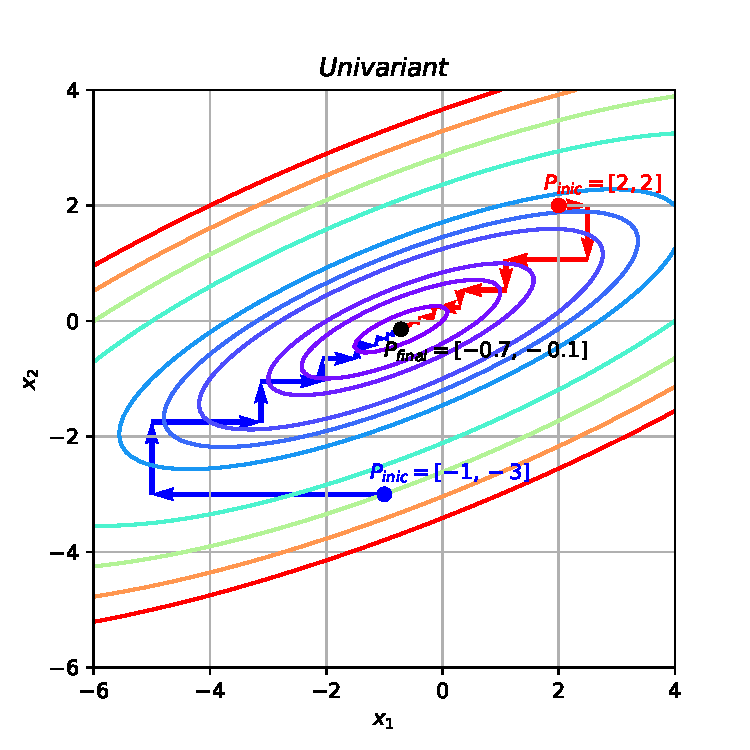
\includegraphics[width=\textwidth]{images/q1a_Univariant.pdf}
      \caption{Univariante}
      \label{fig:q1a_univariant}
  \end{subfigure}
  \hfill
  \begin{subfigure}[b]{0.32\textwidth}
    \centering
    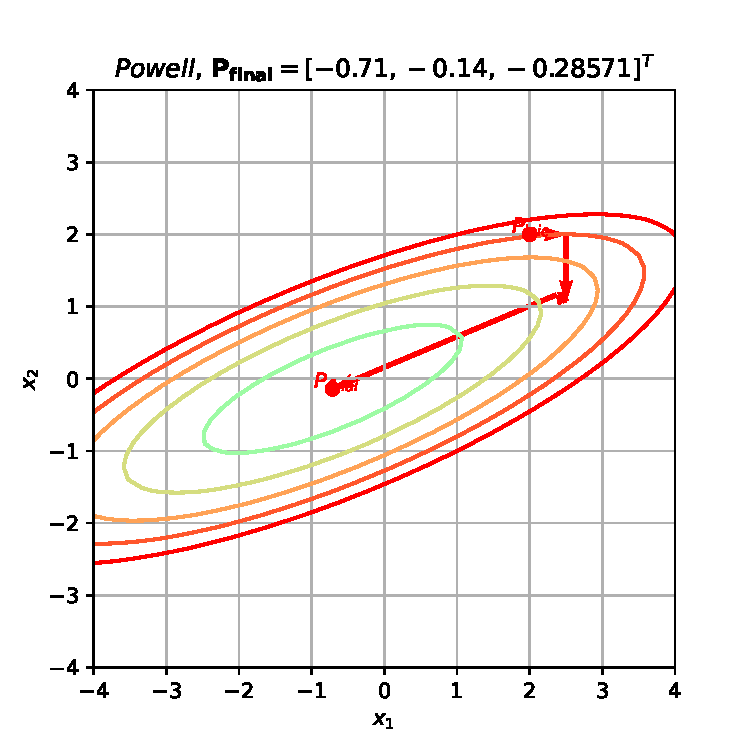
\includegraphics[width=\textwidth]{images/q1a_Powell.pdf}
    \caption{Powell}
    \label{fig:q1a_powell}
  \end{subfigure}
  \hfill
  \begin{subfigure}[b]{0.32\textwidth}
    \centering
    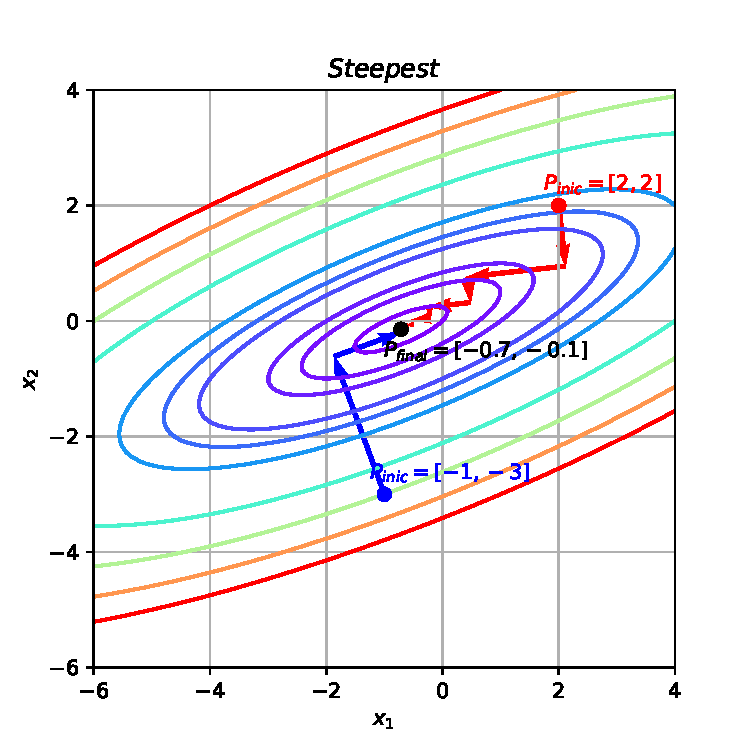
\includegraphics[width=\textwidth]{images/q1a_Steepest.pdf}
    \caption{Steepest Descent}
    \label{fig:q1a_steepest}
  \end{subfigure}
  \hfill
  \begin{subfigure}[b]{0.32\textwidth}
    \centering
    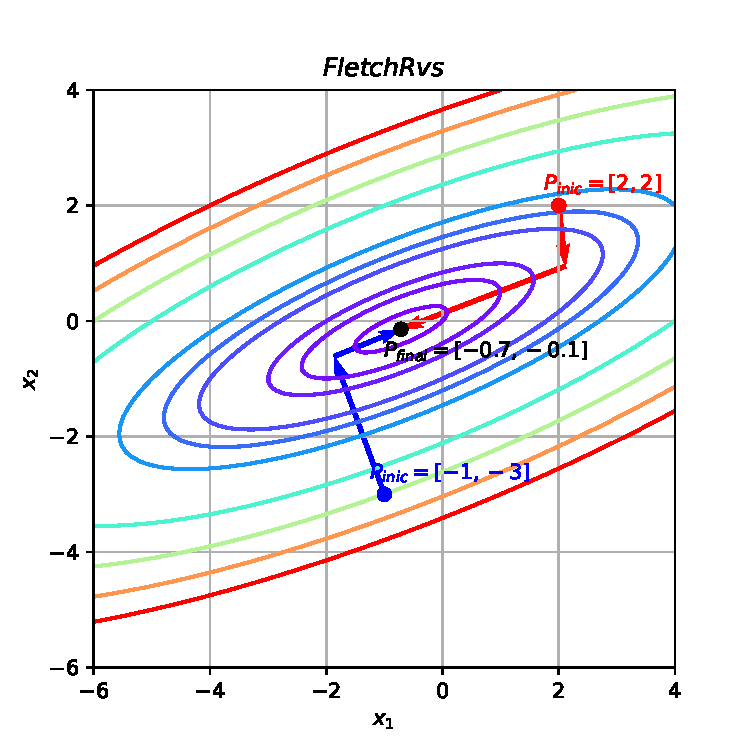
\includegraphics[width=\textwidth]{images/q1a_FletchRvs.pdf}
    \caption{Fletcher-Reeves}
    \label{fig:q1a_fletchrvs}
  \end{subfigure}
  \hfill
  \begin{subfigure}[b]{0.32\textwidth}
    \centering
    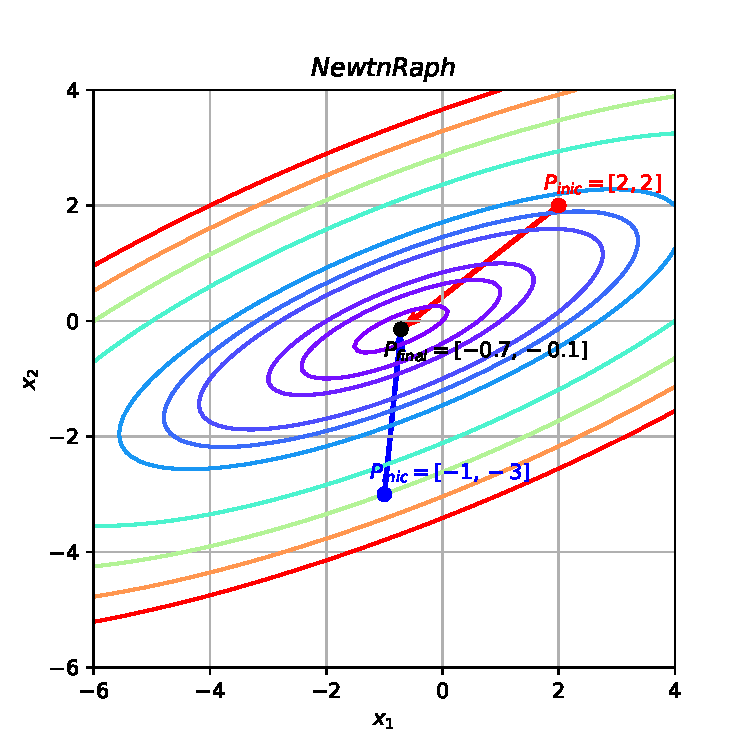
\includegraphics[width=\textwidth]{images/q1a_NewtnRaph.pdf}
    \caption{Newton-Raphson}
    \label{fig:q1a_newtnraph}
  \end{subfigure}
  \hfill
  \begin{subfigure}[b]{0.32\textwidth}
    \centering
    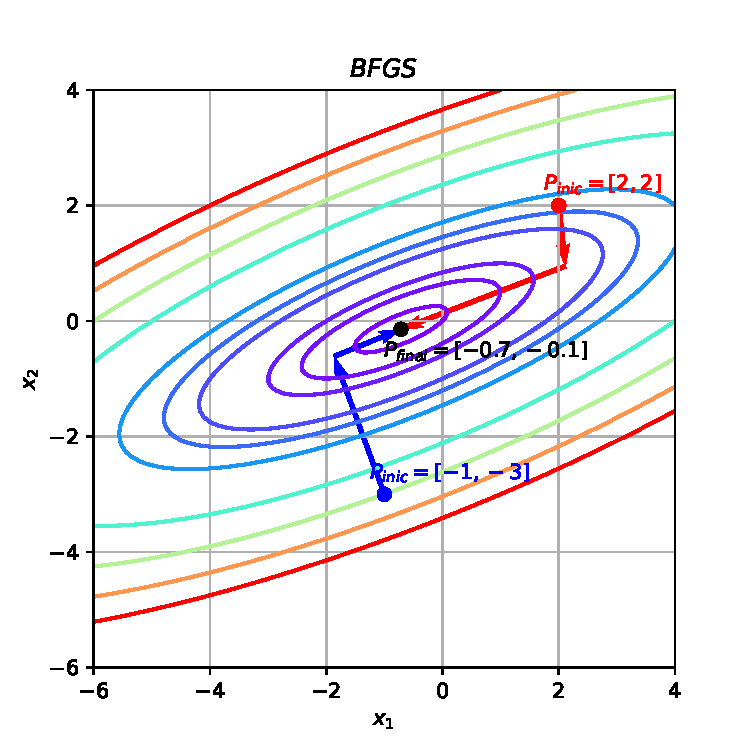
\includegraphics[width=\textwidth]{images/q1a_BFGS.pdf}
    \caption{BFGS}
    \label{fig:q1a_bfgs}
  \end{subfigure}
     \caption{Resultados gráficos para a função \ref{func:a}}
     \label{fig:q1a}
\end{figure}

\subsubsection{Item \ref{func:b}}

Um resumo dos resultados obtidos para o estudo do presente item estão resumidos na Tabela \ref{tab:q1b_results}.
Neste caso, é interessante notar que para os diferentes pontos iniciais, a otimização convergiu para valores de mínimos
distintos, o que é esperado caso os pontos iniciais tenham mínimos locais distintos em suas vizinhanças. 
A Figura \ref{fig:q1b} apresenta visualização gráfica disso ao mostrar que ambos os pontos inicialis tem mínimos distintos
em sua vizinhança, e como os métodos de OSR aqui estudados tem como critério de parada a chegada a um ponto crítico, é esperado
que o mínimo mais próximo do ponto inicial seja a resposta do problema.

\begin{table}[htpb]
  \centering
  \begin{tabular}{|l|c|c|c|c|c|c|c|}
    %\cline{2-7}
    \multicolumn{1}{c}{} %\vline
    & 
    \multicolumn{3}{c}{$\mathbf{x^0} = [10, 2]^T$} \vline
    & 
    \multicolumn{3}{c}{$\mathbf{x^0} = [-2, -3]^T$} \\%\vline \\
    \hline%\cline{2-5}
    \textbf{Método}
    &
    \textbf{Ponto de mínimo}
    & 
    $\mathbf{n}_{passos}$
    & 
    \textbf{t (s)}
    &
    \textbf{Ponto de mínimo}
    & 
    $\mathbf{n}_{passos}$
    & 
    \textbf{t (s)}
    \\
    Univariante        & $[13.000001, 3.999999]^T$ & 65 & 0.019 &  $[7.000001, -2.000001]^T$ &  61  & 0.018    \\
    Powell             & $[13.000001, 4.000000]^T$ & 15 & 0.011 &  $[7.000000, -2.000000]^T$ &  18  & 0.032    \\
    Steepest Descent   & $[13.000002, 3.999999]^T$ & 47 & 0.013 &  $[7.000002, -2.000002]^T$ &  42  & 0.009    \\
    Fletcher-Reeves    & $[13.000001, 3.999999]^T$ & 64 & 0.013 &  $[7.000000, -2.000000]^T$ &  21  & 0.004    \\
    Newton-Raphson     & $[10.000000, 1.000000]^T$ & 1  & 0.001 &  $[7.000000, -2.000000]^T$ &  6   & 0.005    \\
    BFGS               & $[13.000000, 4.000000]^T$ & 9  & 0.008 &  $[7.000000, -2.000000]^T$ &  8   & 0.010    \\
    \hline
  \end{tabular}
  \caption{Resumo dos resultados obtidos para a função (\ref{func:b})}
  \label{tab:q1b_results}
\end{table}

Outro ponto relevante diz respeito ao valor final atingido pelo método de Newton-Raphson, que diverge dos demais métodos para o mesmo
ponto inicial. Novamente, a combinação da análise da direção inicial do método de Newton com o critério de parada, que encerra o processo
em pontos críticos, nos leva a entender que para esse método o ponto final atingido foi um ponto de sela que, embora não seja um mínimo,
também satisfaz o critério de parada.

\begin{figure}[htpb]
  \centering
  \begin{subfigure}[b]{0.32\textwidth}
      \centering
      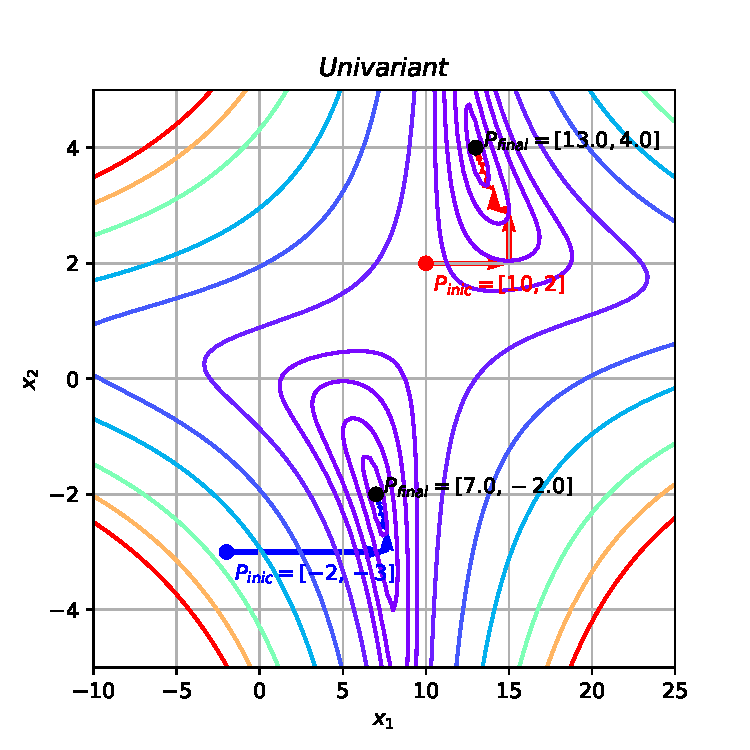
\includegraphics[width=\textwidth]{images/q1b_Univariant.pdf}
      \caption{Univariante}
      \label{fig:q1b_univariant}
  \end{subfigure}
  \hfill
  \begin{subfigure}[b]{0.32\textwidth}
    \centering
    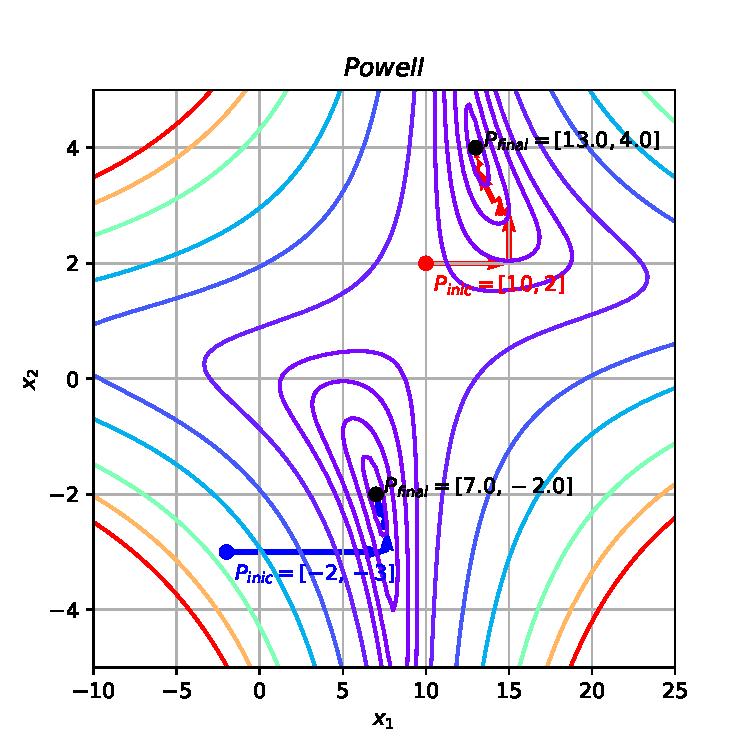
\includegraphics[width=\textwidth]{images/q1b_Powell.pdf}
    \caption{Powell}
    \label{fig:q1b_powell}
  \end{subfigure}
  \hfill
  \begin{subfigure}[b]{0.32\textwidth}
    \centering
    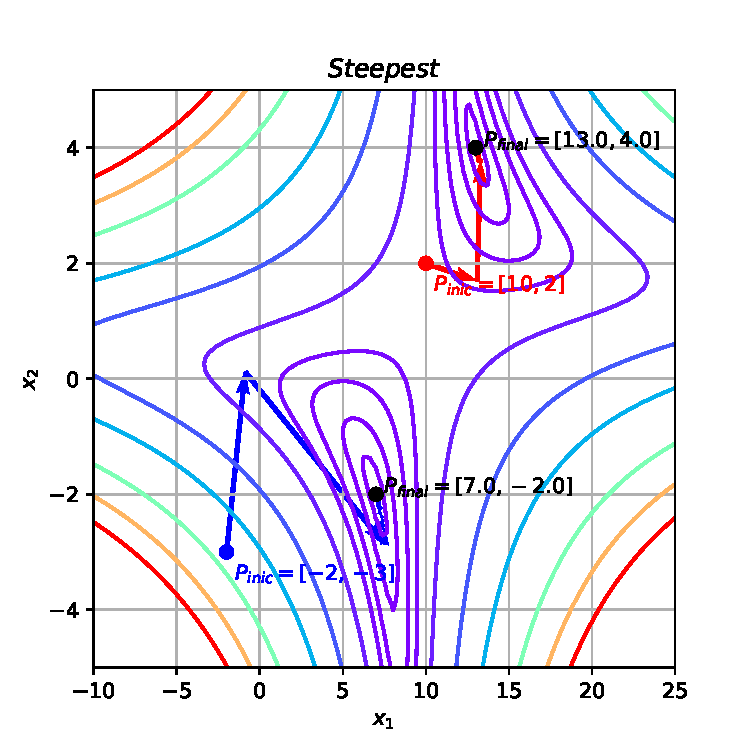
\includegraphics[width=\textwidth]{images/q1b_Steepest.pdf}
    \caption{Steepest Descent}
    \label{fig:q1b_steepest}
  \end{subfigure}
  \hfill
  \begin{subfigure}[b]{0.32\textwidth}
    \centering
    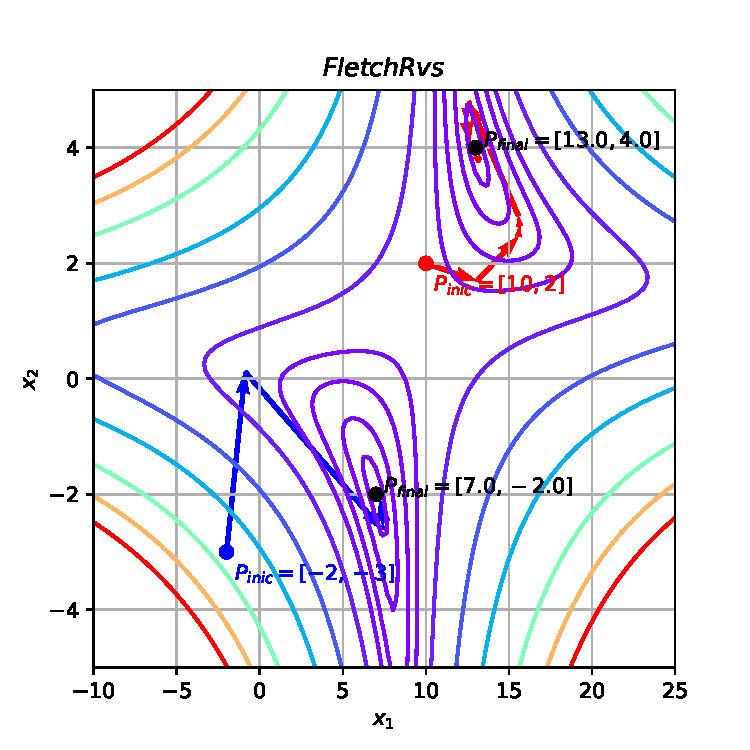
\includegraphics[width=\textwidth]{images/q1b_FletchRvs.pdf}
    \caption{Fletcher-Reeves}
    \label{fig:q1b_fletchrvs}
  \end{subfigure}
  \hfill
  \begin{subfigure}[b]{0.32\textwidth}
    \centering
    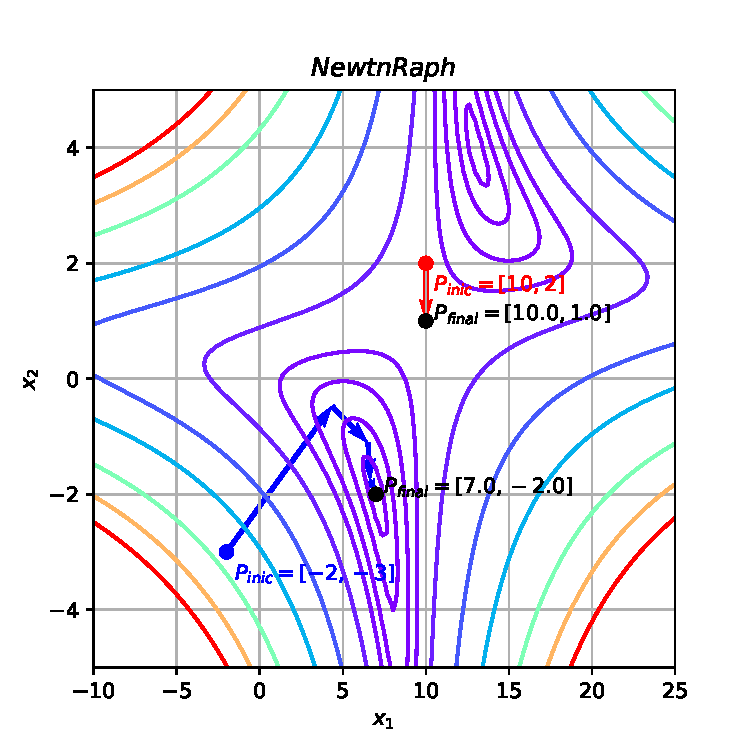
\includegraphics[width=\textwidth]{images/q1b_NewtnRaph.pdf}
    \caption{Newton-Raphson}
    \label{fig:q1b_newtnraph}
  \end{subfigure}
  \hfill
  \begin{subfigure}[b]{0.32\textwidth}
    \centering
    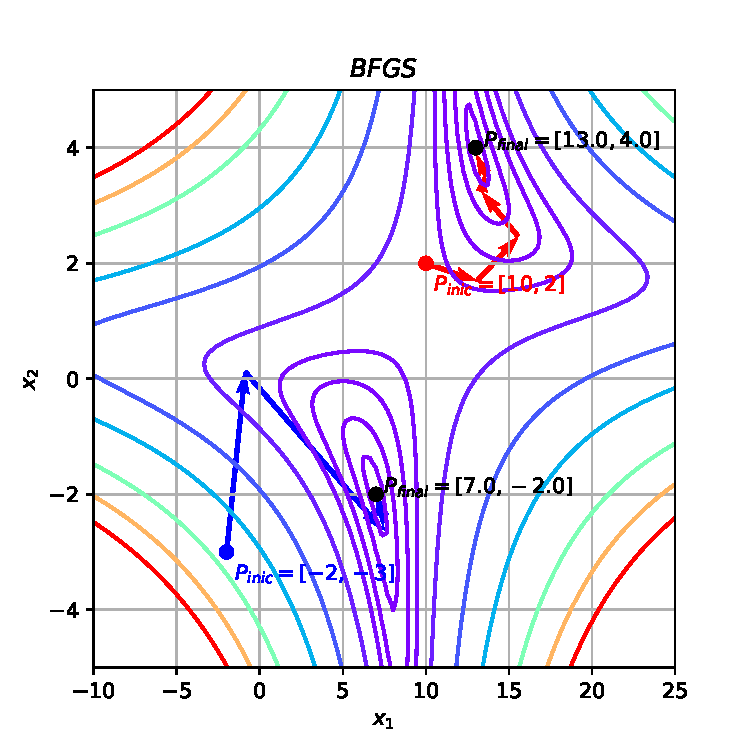
\includegraphics[width=\textwidth]{images/q1b_BFGS.pdf}
    \caption{BFGS}
    \label{fig:q1b_bfgs}
  \end{subfigure}
     \caption{Resultados gráficos para a função \ref{func:b}}
     \label{fig:q1b}
\end{figure}

\section{Questão 02}

\subsection{Enunciado}

Utilizando os métodos de otimização implementados na primeira questão:

\begin{enumerate}[(a)]
  \item Determinar os deslocamentos $(u_A, v_A)$, do ponto $A$, que minimizam a Energia Potencial Total $\Pi$ do sistema de molas indicado na figura abaixo. \
  Adotar o ponto inicial: $x_0 = [0.01, -0.10]^T$. A Figura \ref{fig:q2_schema} exemplifica esse cenário.
  \item desenvolver um estudo de convergência da solução deste problema (i.e., deslocamento do ponto $A$) para níveis crescentes de discretização \
  do modelo (ou seja, considerando o número de molas $n = 2, 4, 6, ...$ ). Se possível, comparar as suas respostas com as soluções obtidas usando o Método \
  dos Elementos Finitos (levando em consideração o comportamento não linear geométrico da estrutura). A rigidez de cada mola ($k_i = 1, ..., n$) é obtida como a \
  razão entre o módulo de rigidez axial do material e o seu comprimento. Os valores $W_j$ (com $j = 1, ..., n$) correspondem às cargas nodais equivalentes aos pesos \
  das molas.
\end{enumerate}

\begin{figure}[htpb]
  \centering
  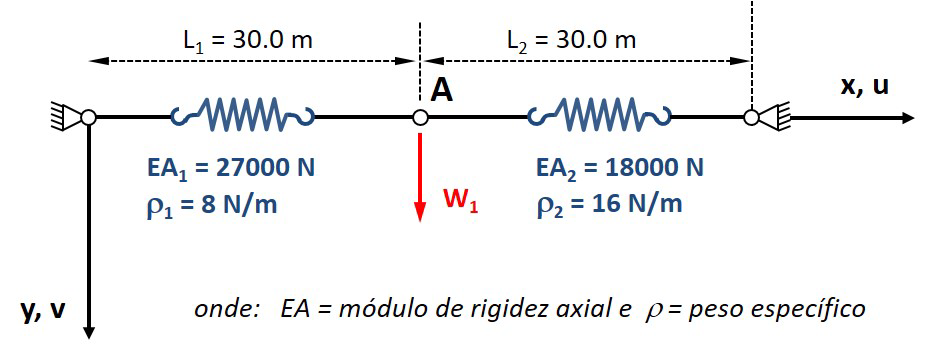
\includegraphics[width=0.8\textwidth]{images/molas.png}
  \caption{Esquemático do problema de duas molas}
  \label{fig:q2_schema}
\end{figure}

\subsection{Solução}

\subsubsection{Determinação do mínimo}

A determinação do deslocamento final do ponto de conexão entre as duas molas pode ser determinado por meio da minimização da energia potencial do sistema,
dada pela equação \ref{eq:q2a} onde $x_1$ é o deslocamento horizontal positivo do ponto e $x_2$ é o deslocamento vertical negativo do mesmo:

\begin{equation}\label{eq:q2a}
  \Pi = \frac{EA_{1} \left(- L_{1} + \sqrt{x_{2}^{2} + \left(L_{1} + x_{1}\right)^{2}}\right)^{2}}{2L_{1}} + \frac{EA_{2} \left(- L_{2} + \sqrt{x_{2}^{2} + \left(L_{2} - x_{1}\right)^{2}}\right)^{2}}{2L_{2}} - \frac{x_{2}}{2} \left(L_{1} \rho_{1} + L_{2} \rho_{2}\right)
\end{equation}

Os resultados obtidos pelo processo de minimização são resumidos na Tabela \ref{tab:q2a_results}, onde novamente podemos ver que todos os métodos numéricos
convergiram para o mesmo ponto final salvo erros numéricos. Se destaca, porém, o tempo que o método de Powell levaou para convergir (aproximadamente 1 min).
Novamente isso parece estar relacionado com a determinação de direções conjugadas de módulo pequeno, o que prejudica a performance da busca linear pelo mínimo.

\begin{table}[htpb]
  \centering
  \begin{tabular}{|l|c|c|c|}
    %\cline{2-4}
    \multicolumn{1}{c}{} %\vline
    & 
    \multicolumn{3}{c}{$\mathbf{x^0} = [0.01, -0.10]^T$} \\%\vline \\
    \hline%\cline{2-5}
    \textbf{Método}
    &
    \textbf{Ponto de mínimo}
    & 
    $\mathbf{n}_{passos}$
    & 
    \textbf{t (s)}
    \\
    Univariante        & $[-0.205109, 7.788993]^T$ & 69  &  0.028    \\
    Powell             & $[-0.205109, 7.788993]^T$ & 28  & 58.743    \\
    Steepest Descent   & $[-0.205109, 7.788993]^T$ & 8   &  0.002    \\
    Fletcher-Reeves    & $[-0.205109, 7.788993]^T$ & 70  &  0.017    \\
    Newton-Raphson     & $[-0.205109, 7.788993]^T$ & 200 &  0.063    \\
    BFGS               & $[-0.205109, 7.788993]^T$ & 200 &  0.055    \\
    \hline
  \end{tabular}
  \caption{Resumo dos resultados obtidos para a discretização em 2 molas}
  \label{tab:q2a_results}
\end{table}


Outro ponto importante é a análise do número de iterações dos métodos de Newton-Raphson e BFGS. Como 200 iterações foi o valor máximo passado para os métodos,
isso indica que ambos não convergiram para este problema. Comparando resultados do ponto final, fica evidente que eles atingiram valores próximos dos demais métodos,
com a não convergência sendo apenas uma questão de o gradiente ter se mantido com módulo acima da tolerância. Espera-se que, caso a tolerência seja relaxada (de $10^{-5}$ para $10^{-4}$,
por exemplo), esses métodos venham a convergir.

A Figura \ref{fig:q2a} mostra as curvas de nível para o problema estudado.

\begin{figure}[htpb]
  \centering
  \begin{subfigure}[b]{0.32\textwidth}
      \centering
      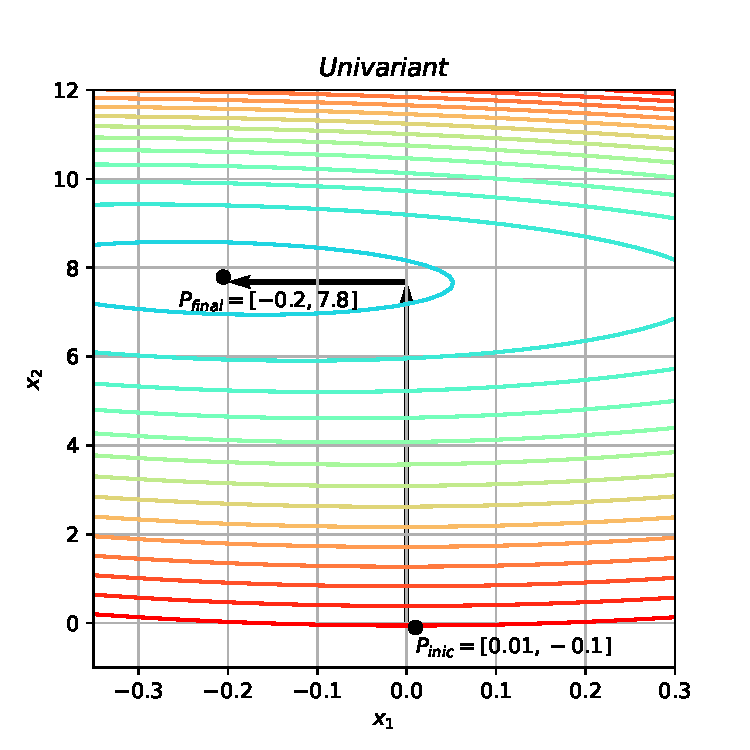
\includegraphics[width=\textwidth]{images/q2a_Univariant.pdf}
      \caption{Univariante}
      \label{fig:q2a_univariant}
  \end{subfigure}
  \hfill
  \begin{subfigure}[b]{0.32\textwidth}
    \centering
    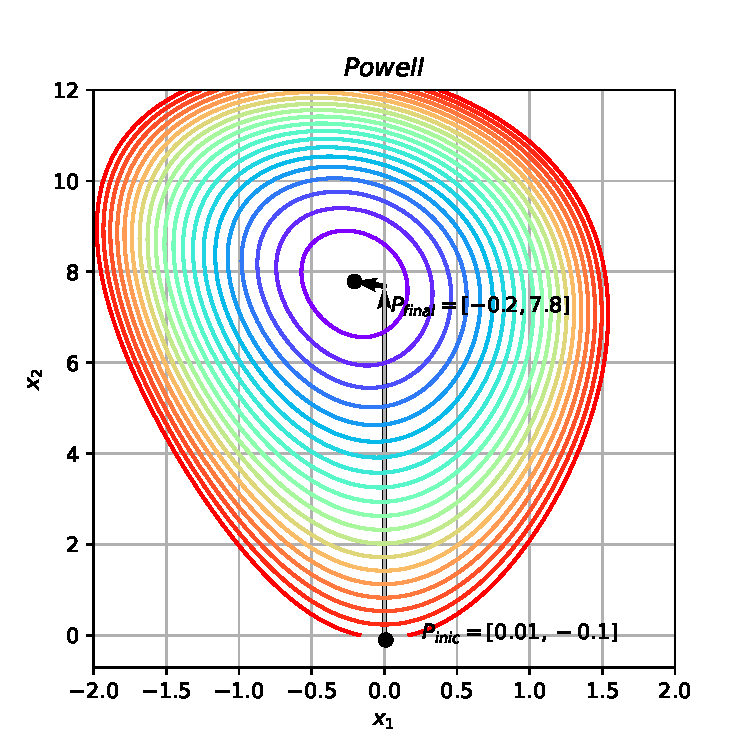
\includegraphics[width=\textwidth]{images/q2a_Powell.pdf}
    \caption{Powell}
    \label{fig:q2a_powell}
  \end{subfigure}
  \hfill
  \begin{subfigure}[b]{0.32\textwidth}
    \centering
    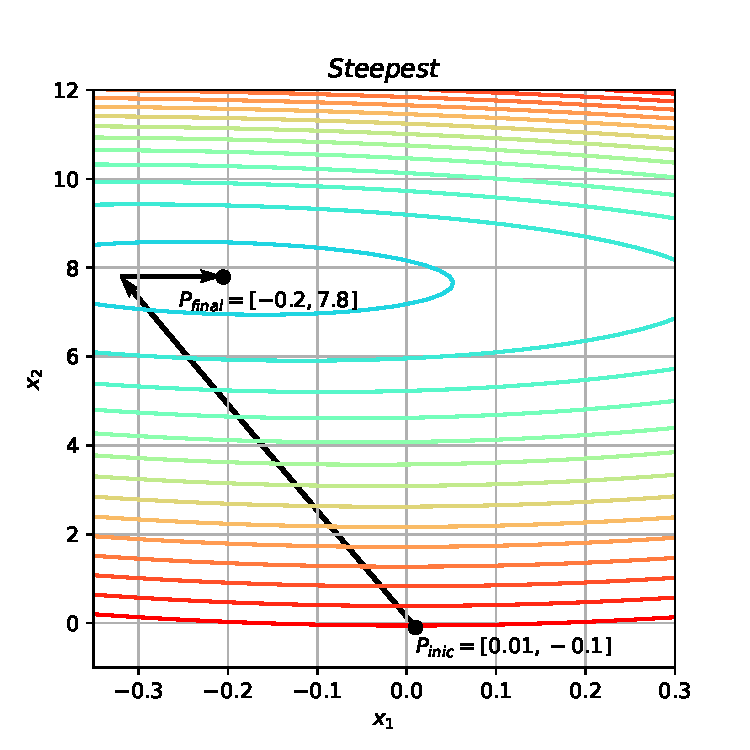
\includegraphics[width=\textwidth]{images/q2a_Steepest.pdf}
    \caption{Steepest Descent}
    \label{fig:q2a_steepest}
  \end{subfigure}
  \hfill
  \begin{subfigure}[b]{0.32\textwidth}
    \centering
    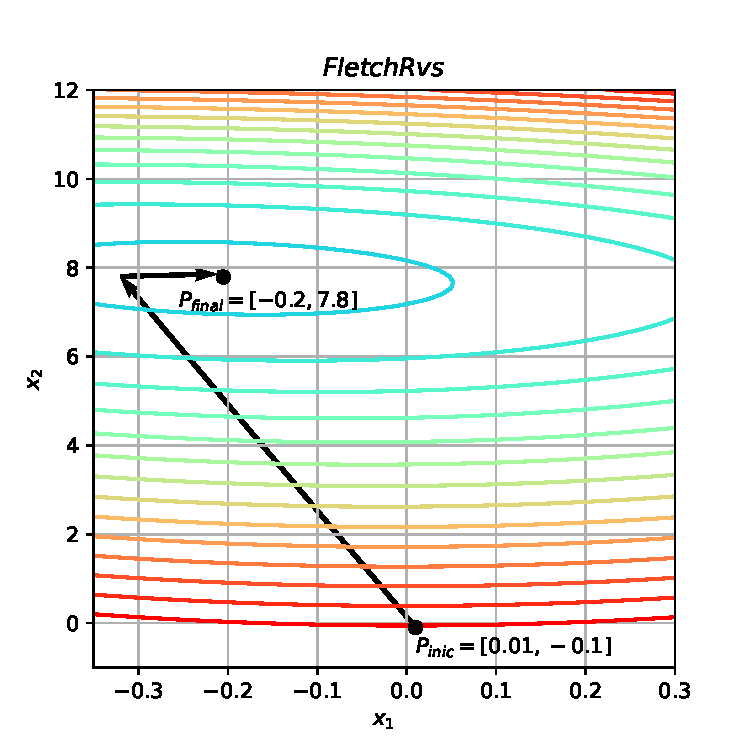
\includegraphics[width=\textwidth]{images/q2a_FletchRvs.pdf}
    \caption{Fletcher-Reeves}
    \label{fig:q2a_fletchrvs}
  \end{subfigure}
  \hfill
  \begin{subfigure}[b]{0.32\textwidth}
    \centering
    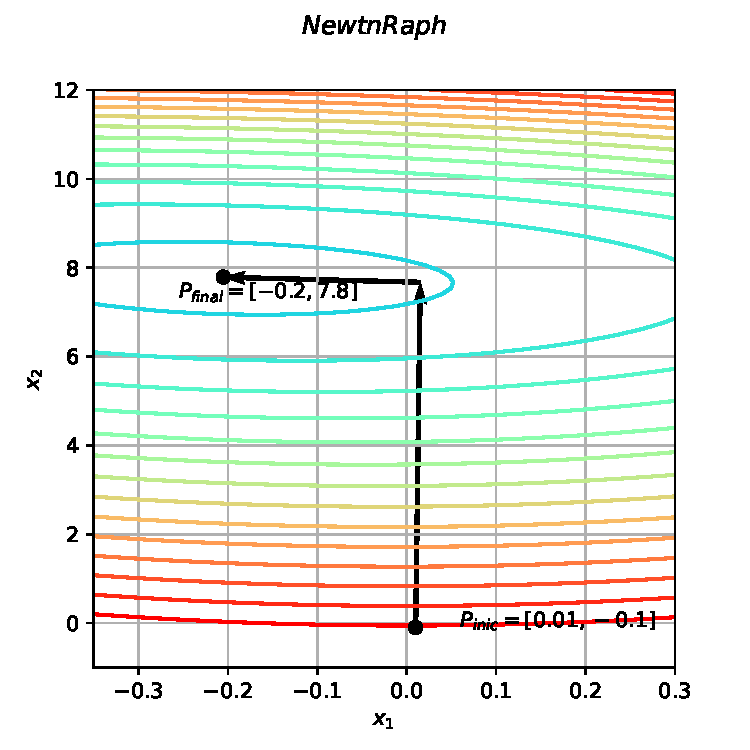
\includegraphics[width=\textwidth]{images/q2a_NewtnRaph.pdf}
    \caption{Newton-Raphson}
    \label{fig:q2a_newtnraph}
  \end{subfigure}
  \hfill
  \begin{subfigure}[b]{0.32\textwidth}
    \centering
    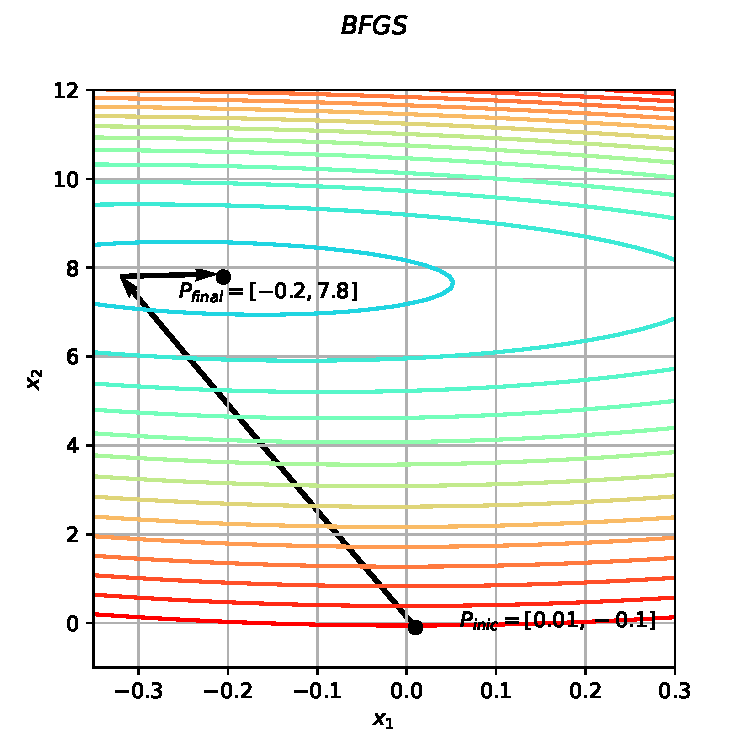
\includegraphics[width=\textwidth]{images/q2a_BFGS.pdf}
    \caption{BFGS}
    \label{fig:q2a_bfgs}
  \end{subfigure}
     \caption{Resultados gráficos da determinação do mínimo da função potencial}
     \label{fig:q2a}
\end{figure}

\subsubsection{Análise de convergência}

O estudo de análise de convergência tem por objetivo analisar a escalabilidade dos métodos implementados
para funções de mais de duas direções e também avaliar o impacto dessa alta dimensionalidade na performance dos
métodos de otimização. Para tal, uma formulação mais genérica do problema precisou ser elaborada.

Suponha uma mola individual $i$, caracterizada pelas propriedades $EA_i, dL_i, \rho_i$ e com extremos nos pontos
$[x_{1,i}, x_{2,i}]^T$ e $[x_{1,i+1}, x_{2,i+1}]^T$. A equação \ref{eq:q2b_1} representa a energia potencial dessa mola:

\begin{equation}\label{eq:q2b_1}
  \Pi_i = \frac{EA_{i} \left(- dL_{i} + \sqrt{(x_{2,i+1}-x_{2,i})^{2} + \left(dL_{i} + x_{1,i+1}-x_{1,i}\right)^{2}}\right)^{2}}{2dL_{i}}  - \frac{x_{2,i}+x_{2,i+1}}{2} \left(dL_{i} \rho_{i}\right)
\end{equation}

Caso queiramos calcular a energia potencial de $n$ molas com $n+1$ nós (incluindo extremos) que componham a totalidade
da nossa mola discretizada, a energia potencial total será dada pela expressão \ref{eq:q2b_2}:

\begin{equation}\label{eq:q2b_2}
  \Pi = \sum_{i-1}^n \Pi_i
\end{equation}

Para a realização desse estudo e dada a complexidade crescente do problema, algumas alterações nos parâmetros
de otimização foram feitas:

\begin{itemize}
  \item Número máximo de iterações foi para 500
  \item Tolerância da norma do gradiente aumentada para $10^{-3}$
  \item Normalização da direção na busca linear
  \item Passo constante inicial $\Delta\alpha = 0.001$
  \item Ponto inicial padronizado em $\mathbf{x_0} = \mathbf{0}$
\end{itemize}

Além disso, devido à complexidade de se obter gradiente e Hessiana analíticos para o problema, a interface {\tt NumericalSpecialFunction},
com derivação numérica, foi usada para este problema. A convergência, por sua vez, foi estudada para a discretização de cada mola do par que
compõe o problema em 1, 2, 4, 6 e 8 molas, garantindo sempre a simetria de nós com relação ao centro.

Os resultados obtidos para a análise de convergência podem ser vistos na Tabela \ref{tab:q2b_results}, com casos em que não houve convergência
em 500 passos sinalizados em vermelho. Em termos de performance é possível ver que, para números de iterações relativamente grandes, o aumento
da dimensionalidade do problema está intrinsecamente ligado ao aumento do tempo computacional gasto pelo método. Outro fator interessante de
se notar vem da comparação do método de Newton-Raphson com BFGS, em que fica claro que o segundo, mesmo com mais iterações que o primeiro, demandou
um tempo computacional menor ou igual em praticamente todos os casos, o que provavelmente está associado ao alto custo de se estimar numericamente a Hessiana
de problemas de grande dimensionalidade.

\begin{table}[htpb]
  \centering
  \begin{tabular}{|l|c|c|c|c|c|c|c|c|c|c|}
    \multicolumn{1}{c}{}
    &
    \multicolumn{2}{c}{1 mola} \vline
    &
    \multicolumn{2}{c}{2 molas} \vline
    &
    \multicolumn{2}{c}{4 molas} \vline
    &
    \multicolumn{2}{c}{6 molas} \vline
    &
    \multicolumn{2}{c}{8 molas}
    \\
    \hline%\cline{2-5}
    \textbf{Método}
    &
    $\mathbf{n}_{passos}$
    & 
    \textbf{t (s)}
    &
    $\mathbf{n}_{passos}$
    & 
    \textbf{t (s)}
    &
    $\mathbf{n}_{passos}$
    & 
    \textbf{t (s)}
    &
    $\mathbf{n}_{passos}$
    & 
    \textbf{t (s)}
    &
    $\mathbf{n}_{passos}$
    & 
    \textbf{t (s)}
    \\
    Univariante        &  9 &  0.287  &  152 & 1.709 & {\color{red} 500} & 9.800 & {\color{red} 500} & 18.540 & {\color{red} 500} & 29.059 \\
    Powell             & 13 &  0.282  &  {\color{red} 500} & 3.661 & {\color{red} 500} & 9.739 & {\color{red} 500} & 17.908 & {\color{red} 500} & 28.633 \\
    Steepest           &  8 &  0.282  &  454 & 3.089 & {\color{red} 500} & 8.708 & {\color{red} 500} & 15.931 & {\color{red} 500} & 24.517 \\
    Fletcher           &  9 &  0.274  &   58 & 0.902 & 178 & 4.045 & 301 & 10.859 & 419 & 22.782 \\
    Newton             &  3 &  0.271  &    6 & 0.788 &   7 & 2.489 &   8 &  7.538 &   9 & 15.537 \\
    BFGS               &  4 &  0.270  &   13 & 0.681 &  26 & 1.766 &  38 &  3.298 &  47 &  5.384 \\
    \hline
  \end{tabular}
  \caption{Resumo dos resultados obtidos para a discretização em n molas}
  \label{tab:q2b_results}
\end{table}

Os resultados finais podem ser vistos na Figura \ref{fig:q2b}. É importante notar que os métodos em vermelho não convergiram em
todos os casos, apresentando geometrias finais estranhas. A princípio isso não indica uma impossibilidade de se usar estes métodos
para o probblema estudado, mas indica apenas que eles demandariam um número maior de iterações e mais custo computacional para atingir
a mesma performance dos métodos que convergiram.

\begin{figure}[htpb]
  \centering
  \begin{subfigure}[b]{0.32\textwidth}
      \centering
      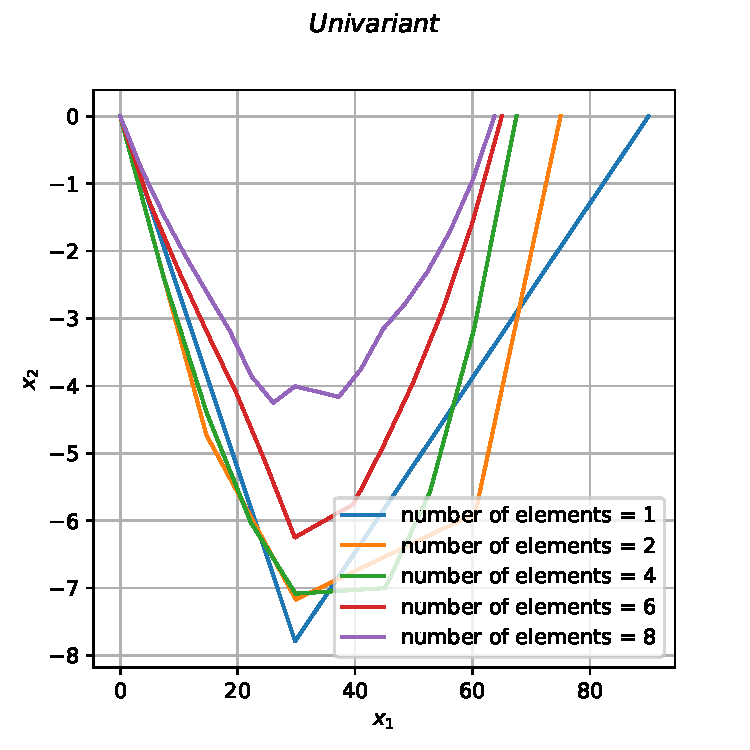
\includegraphics[width=\textwidth]{images/q2b_Univariant.pdf}
      \caption{{\color{red} Univariante}}
      \label{fig:q2b_univariant}
  \end{subfigure}
  \hfill
  \begin{subfigure}[b]{0.32\textwidth}
    \centering
    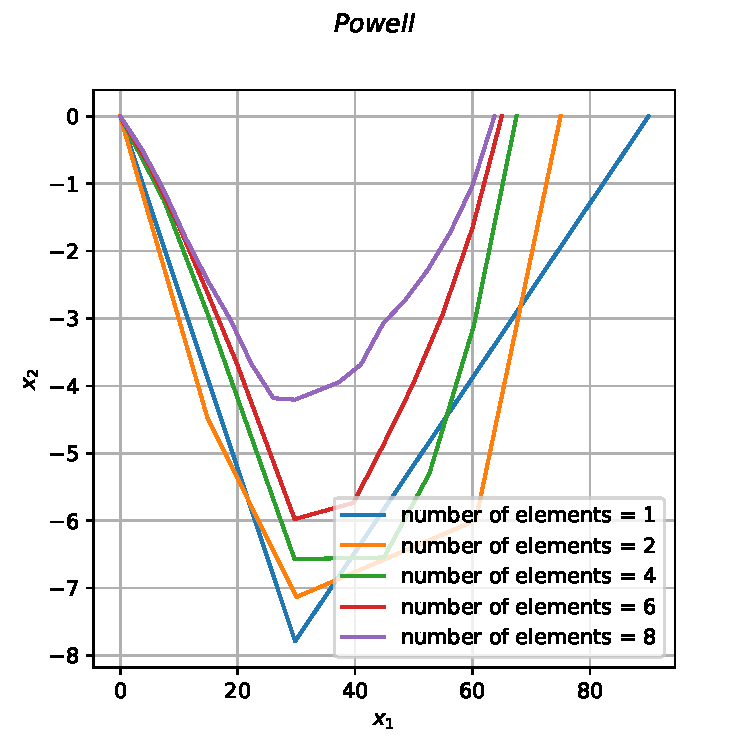
\includegraphics[width=\textwidth]{images/q2b_Powell.pdf}
    \caption{{\color{red} Powell}}
    \label{fig:q2b_powell}
  \end{subfigure}
  \hfill
  \begin{subfigure}[b]{0.32\textwidth}
    \centering
    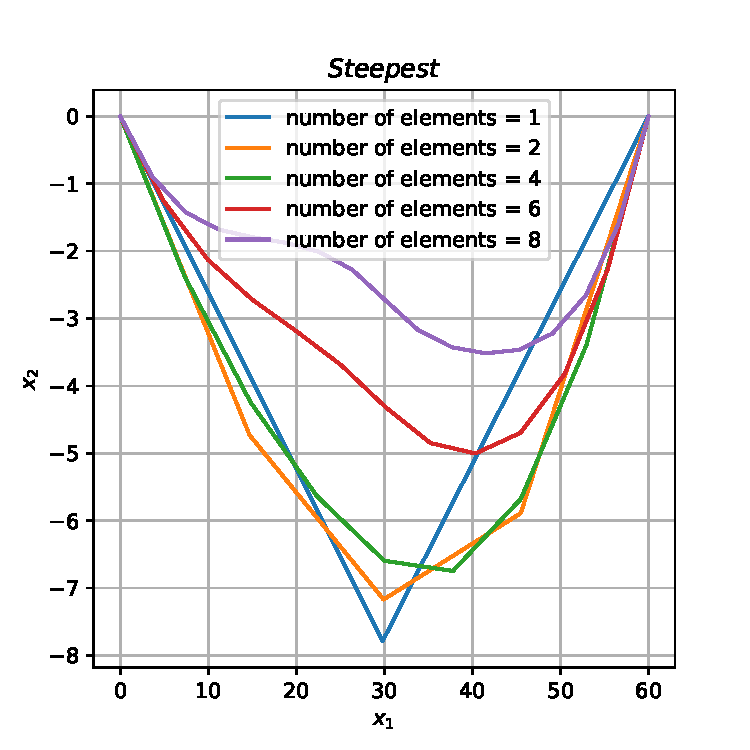
\includegraphics[width=\textwidth]{images/q2b_Steepest.pdf}
    \caption{{\color{red} Steepest Descent}}
    \label{fig:q2b_steepest}
  \end{subfigure}
  \hfill
  \begin{subfigure}[b]{0.32\textwidth}
    \centering
    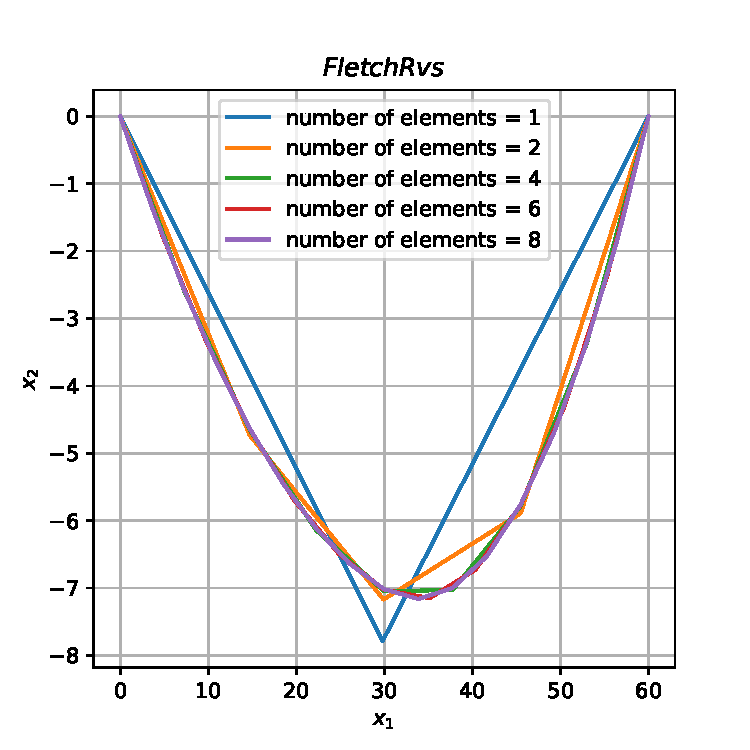
\includegraphics[width=\textwidth]{images/q2b_FletchRvs.pdf}
    \caption{Fletcher-Reeves}
    \label{fig:q2b_fletchrvs}
  \end{subfigure}
  \hfill
  \begin{subfigure}[b]{0.32\textwidth}
    \centering
    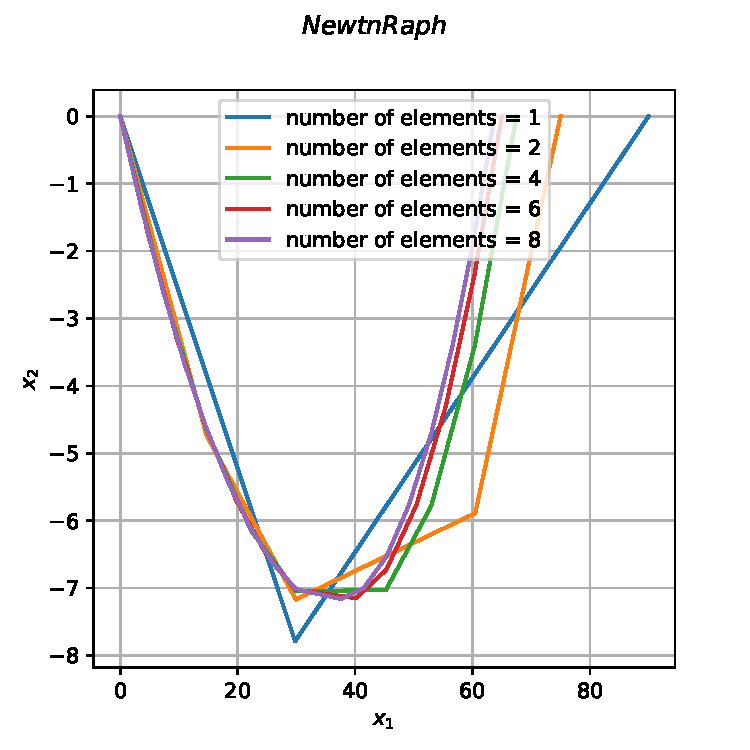
\includegraphics[width=\textwidth]{images/q2b_NewtnRaph.pdf}
    \caption{Newton-Raphson}
    \label{fig:q2b_newtnraph}
  \end{subfigure}
  \hfill
  \begin{subfigure}[b]{0.32\textwidth}
    \centering
    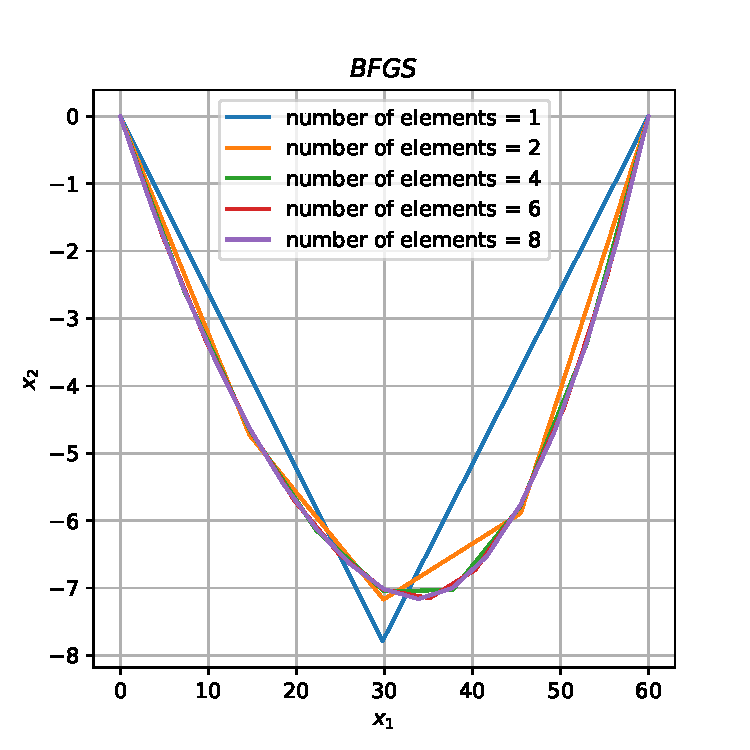
\includegraphics[width=\textwidth]{images/q2b_BFGS.pdf}
    \caption{BFGS}
    \label{fig:q2b_bfgs}
  \end{subfigure}
     \caption{Resultados da análise de convergência para discretizações maiores da mola}
     \label{fig:q2b}
\end{figure}

%%%%%%%%%%%%%%%%%%%%%%%%%%%%%%%%%%%%%%%%%%%%%%%%%%%

\bibliographystyle{apalike}
\bibliography{export}

\end{document}